\documentclass[12pt]{article}
\usepackage[utf8]{inputenc}
\usepackage[T1]{fontenc}
\usepackage{graphicx}
\usepackage{subcaption}
\usepackage{amsmath}
\usepackage{fancyhdr}
\usepackage{geometry}
\usepackage[english]{babel}
\usepackage{csquotes}
\usepackage{hyperref}
\usepackage{url}
\usepackage{listings}
\usepackage{float}
\usepackage{booktabs}
\usepackage{array}
\usepackage{tikz}
\usetikzlibrary{
    shapes.geometric, shapes.misc,
    arrows.meta, positioning, fit,
    backgrounds, calc, decorations.pathreplacing,
    automata
}
\usepackage{setspace}

\lstset{
    language=C,
    basicstyle=\ttfamily\small,
    numberstyle=\tiny,
    frame=single,
    breaklines=true,
}

% ── TikZ styles ────────────────────────────────────────────────────────────────
\tikzset{
  comp/.style={rectangle, draw, rounded corners=3pt,
               minimum width=2.8cm, minimum height=0.75cm,
               align=center, font=\small},
  hw/.style={comp, fill=gray!20},
  driver/.style={comp, fill=blue!15},
  service/.style={comp, fill=green!15},
  task/.style={comp, fill=orange!20},
  app/.style={comp, fill=yellow!20},
  arr/.style={-Stealth, thick},
  biarr/.style={Stealth-Stealth, thick},
  layer/.style={rectangle, draw, minimum height=0.9cm,
                align=center, font=\small\bfseries},
  cls/.style={rectangle, draw, font=\small, text width=2.8cm,
              minimum width=3.0cm, inner sep=3pt},
  hdr/.style={cls, fill=gray!10, align=center, font=\small\bfseries},
  uses/.style={-Stealth, dashed, thick},
  impl/.style={-Stealth, thick},
  state/.style={circle, draw, fill=blue!10, minimum size=2.0cm,
                align=center, font=\small\bfseries},
}
% ───────────────────────────────────────────────────────────────────────────────

\linespread{1.25}
\setlength{\parindent}{0.8cm}
\setlength{\parskip}{0em}
\renewcommand{\headrulewidth}{0pt}
\geometry{a4paper, portrait, margin=1in}
\setlength{\headheight}{14.49998pt}

\begin{document}
\begin{titlepage}
   \begin{center}
    \textsc{\large Ministry of Education of Republic of Moldova}\\[0.5cm]
    \textsc{\large Technical University of Moldova}\\[0.5cm]
    \textsc{\large Faculty of Computers, Informatics and Microelectronics}\\[0.5cm]
    \textsc{\large Software Engineering Department}\\[1.2cm]

    \vspace{25mm}

    {\LARGE \textbf{\textsc{Embedded Systems}}}\\[0.5cm]
    \textsc{\large Laboratory No. 1.6}\\[0.5cm]

    \newcommand{\HRule}{\rule{\linewidth}{0.5mm}}
    \vspace{80mm}

    \begin{minipage}[t]{0.4\textwidth}
    \begin{flushleft} \large
    \emph{Author:} \\
    Vladimir \textsc{Vitcovschii}\\
    std. gr. FAF-231
    \end{flushleft}
    \end{minipage}
    ~
    \begin{minipage}[t]{0.4\textwidth}
    \begin{flushright} \large
    \end{flushright}
    \end{minipage}\\[3cm]

    \vspace{5mm}
    \large Chi\c{s}in\u{a}u 2026\\[0.5cm]

    \vfill
    \end{center}
\end{titlepage}

\clearpage
\tableofcontents
\clearpage

\setcounter{page}{2}
\pagestyle{fancy}
\fancyhf{}
\rhead{\thepage}
\lhead{FAF-231 Vitcovschii Vladimir; Laboratory Work No. 1.6}

% ─────────────────────────────────────────────────────────────────────────────
\section{The Purpose of the Work}
% ─────────────────────────────────────────────────────────────────────────────

The purpose of this laboratory work is to develop an analog signal conditioning pipeline using FreeRTOS on an ATmega2560 microcontroller. The application reads an NTC thermistor sensor and passes the raw ADC value through a multi-stage conditioning chain --- saturation (clamping), median filtering, and weighted moving average --- before converting the conditioned value to temperature via the Steinhart--Hart equation. The focus is on understanding each conditioning stage's role in producing a clean, reliable measurement from a noisy analog input.

% ─────────────────────────────────────────────────────────────────────────────
\section{Objectives of the Work}
% ─────────────────────────────────────────────────────────────────────────────

The task requires implementing an analog signal conditioning system on an ATmega2560 with FreeRTOS, using three concurrent tasks:
\begin{itemize}
  \item \textbf{Task~1 --- Sensor Reader}: Read the NTC thermistor via ADC every 50\,ms and store the raw value in shared memory under mutex protection. Signal the conditioning task via a binary semaphore.
  \item \textbf{Task~2 --- Signal Conditioner}: Wait for each new sample (event-driven via semaphore), then apply the conditioning pipeline: saturation [150--900] $\to$ median filter [window~5] $\to$ weighted moving average [weights: 50, 25, 15, 10] $\to$ Steinhart--Hart temperature conversion. Determine alert status and control LEDs.
  \item \textbf{Task~3 --- Display}: Every 500\,ms, snapshot all pipeline intermediate values and emit a formatted status line via \texttt{printf\_P}.
  \item Use a mutex (\texttt{xLab6Mutex}) for shared data protection and a binary semaphore (\texttt{xLab6NewSample}) for producer-consumer signalling between the sensor reader and conditioner.
  \item Implement the signal conditioning algorithms as a reusable \texttt{SignalConditioner} module.
  \item All configuration values (pins, saturation limits, filter sizes, weights, timing) must be named constants.
\end{itemize}

% ─────────────────────────────────────────────────────────────────────────────
\section{Domain Analysis}
% ─────────────────────────────────────────────────────────────────────────────

\subsection{Signal Conditioning Pipeline}

Raw ADC readings from an analog sensor are subject to noise, outliers, and out-of-range values. A signal conditioning pipeline applies successive transformations to produce a clean, reliable measurement. The pipeline used in this application consists of three stages:

\begin{enumerate}
  \item \textbf{Saturation (Clamping)}: Restricts the ADC value to a valid operating range $[V_{min}, V_{max}]$. Values below $V_{min}$ are clamped to $V_{min}$; values above $V_{max}$ are clamped to $V_{max}$. This rejects readings from disconnected or shorted sensors.
  \item \textbf{Median Filter}: Selects the median value from a sliding window of $N$ recent samples. The median is robust against impulse noise (salt-and-pepper spikes) because a single outlier cannot shift the median.
  \item \textbf{Weighted Moving Average}: Computes a weighted sum of the $K$ most recent median-filtered values. More recent samples receive higher weights, providing temporal smoothing while maintaining responsiveness to genuine changes.
\end{enumerate}

\begin{equation}
\text{Pipeline: } \underbrace{ADC}_{\text{raw}} \xrightarrow{\text{Saturate}} \underbrace{[150, 900]}_{\text{clamped}} \xrightarrow{\text{Median}_5} \underbrace{x_{med}}_{\text{filtered}} \xrightarrow{\text{WAvg}_{4}} \underbrace{x_{avg}}_{\text{smoothed}} \xrightarrow{\text{S-H}} \underbrace{T\,(^{\circ}\text{C})}_{\text{temperature}}
\label{eq:pipeline}
\end{equation}

\subsection{Saturation (Clamping)}

The saturation function restricts the input to a valid range:
\begin{equation}
y = \begin{cases}
V_{min} & \text{if } x < V_{min} \\
V_{max} & \text{if } x > V_{max} \\
x       & \text{otherwise}
\end{cases}
\label{eq:saturation}
\end{equation}

In this application, $V_{min} = 150$ and $V_{max} = 900$. ADC values outside this range indicate sensor fault conditions (e.g., open or shorted wiring) and are clamped to the boundary values.

\subsection{Median Filter}

Given a window of $N$ samples $\{x_1, x_2, \ldots, x_N\}$, the median filter sorts them and selects the middle element:
\begin{equation}
y = \text{sorted}(x_1, \ldots, x_N)\!\left[\lfloor N/2 \rfloor\right]
\label{eq:median}
\end{equation}

With $N = 5$, the filter can reject up to 2 outlier samples per window while preserving the signal's step response (no blurring of sharp transitions). The implementation uses insertion sort on a local copy to avoid modifying the circular buffer.

\subsection{Weighted Moving Average}

The weighted average of $K$ samples with weights $w_i$:
\begin{equation}
y = \frac{\sum_{i=0}^{K-1} w_i \cdot x_i}{\sum_{i=0}^{K-1} w_i}
\label{eq:wavg}
\end{equation}

The weights $\{50, 25, 15, 10\}$ sum to 100, giving the most recent sample 50\% influence, the second most recent 25\%, and so on. This provides exponential-like decay with a fixed window, balancing noise smoothing against tracking speed.

\subsection{NTC Thermistor and Steinhart--Hart Conversion}

The NTC thermistor and Steinhart--Hart equation are identical to Lab~1.5. The thermistor has $R_0 = 10$\,k$\Omega$ at $T_0 = 25\,^{\circ}$C, $B = 3950$, with a 10\,k$\Omega$ fixed resistor in a voltage divider. The key difference is that the Steinhart--Hart conversion is applied to the \emph{conditioned} ADC value (after saturation, median, and weighted average), not the raw reading.

\subsection{Technology Stack}

\begin{table}[H]
\centering
\begin{tabular}{@{}lll@{}}
\toprule
\textbf{Layer} & \textbf{Technology} & \textbf{Details} \\
\midrule
Hardware Platform    & Arduino Mega 2560  & ATmega2560, 16\,MHz, 5\,V \\
Build System         & PlatformIO         & \texttt{atmelavr} platform, Arduino framework \\
Programming Language & C++                & AVR-GCC toolchain \\
RTOS                 & FreeRTOS 10.5.1    & \texttt{feilipu/FreeRTOS} Arduino library \\
STDIO Hook           & AVR-libc           & \texttt{fdev\_setup\_stream} $\to$ \texttt{SerialStream} \\
Serial Communication & UART0              & 9600\,baud, 8N1 \\
Sensor               & NTC 10\,k$\Omega$  & $B = 3950$, voltage divider with $R_{fixed} = 10$\,k$\Omega$ \\
Simulation           & Wokwi / SimulIDE   & Real-time circuit and firmware simulation \\
\bottomrule
\end{tabular}
\caption{Technology Stack}
\label{tab:techstack}
\end{table}

\subsection{System Elements}

\begin{itemize}
  \item \textbf{Arduino Mega 2560 (ATmega2560)}: 256\,KB flash, 8\,KB SRAM, 16\,MHz. FreeRTOS uses one hardware timer for its tick; the 10-bit ADC provides sensor readings.
  \item \textbf{NTC Thermistor (A0)}: 10\,k$\Omega$ at 25\,$^{\circ}$C, $B = 3950$. Connected in a voltage divider: VCC $\to$ $R_{fixed}$ (10\,k$\Omega$) $\to$ ADC pin (A0) $\to$ NTC $\to$ GND.
  \item \textbf{Green LED (D12)}: Indicates normal state (conditioned temperature below threshold). 220\,$\Omega$ current-limiting resistor.
  \item \textbf{Red LED (D11)}: Indicates alert state (conditioned temperature above threshold). Same resistor topology.
  \item \textbf{Yellow LED (D10)}: Toggles on each conditioning cycle to indicate pipeline activity. 220\,$\Omega$ resistor.
  \item \textbf{PlatformIO}: Build system with \texttt{env:mega\_lab6} environment defining \texttt{-D USE\_FREERTOS -D ACTIVE\_LAB=6}. \cite{pio}
\end{itemize}

% ─────────────────────────────────────────────────────────────────────────────
\section{Design}
% ─────────────────────────────────────────────────────────────────────────────

\subsection{Architectural Design}

% ── Mermaid source (render externally and save as images/lab6_component.png) ──
% ```mermaid
% graph TD
%     subgraph APP["APP Layer"]
%         MainLab6["MainLab6<br/>SetupLab6 / LoopLab6"]
%     end
%     subgraph TASKS["TASKS Layer"]
%         T1["TaskSensorRead6Func<br/>50 ms periodic"]
%         T2["TaskCondition6Func<br/>event-driven"]
%         T3["TaskDisplay6Func<br/>500 ms periodic"]
%     end
%     subgraph SRV["SRV Layer"]
%         SYNC["Lab6Sync<br/>xLab6Mutex<br/>xLab6NewSample<br/>shared volatile data"]
%         CFG["Lab6Config<br/>pins, saturation, weights, timing"]
%         SC["SignalConditioner<br/>Saturation, Median, WAvg"]
%         STDIO["StdioRedirect"]
%     end
%     subgraph ECAL["ECAL Layer"]
%         NTC["NtcSensor<br/>ADC + Steinhart-Hart"]
%         LD["LedDriver"]
%         SS["SerialStream<br/>IStream"]
%     end
%     subgraph HW["HW Layer"]
%         MCU["ATmega2560"]
%         SENSOR["NTC on A0"]
%         LEDS["LEDs D10,D11,D12"]
%         UART["UART0"]
%     end
%     MainLab6 --> T1
%     MainLab6 --> T2
%     MainLab6 --> T3
%     T1 -->|ReadNtcRaw| NTC
%     T1 -->|xLab6Mutex lock| SYNC
%     T1 -->|xSemaphoreGive| SYNC
%     T2 -->|xSemaphoreTake| SYNC
%     T2 -->|xLab6Mutex lock| SYNC
%     T2 -->|ApplySaturation, Median, WAvg| SC
%     T2 -->|NtcAdcToTempC10| NTC
%     T2 -->|SetLedState| LD
%     T3 -->|xLab6Mutex lock| SYNC
%     T3 -->|printf_P| STDIO
%     STDIO --> SS
%     NTC --> MCU
%     LD --> MCU
%     SS --> UART
%     MCU --- SENSOR
%     MCU --- LEDS
%     MCU --- UART
% ```

\begin{figure}[H]
\centering
\includegraphics[width=0.85\textwidth]{images/lab6_component.png}
\caption{Component Diagram --- Analog Signal Conditioning Pipeline}
\label{fig:component}
\end{figure}

Table~\ref{tab:components} summarises the role of each component.

\begin{table}[H]
\centering
\begin{tabular}{@{}p{3.6cm}p{2.8cm}p{6.0cm}@{}}
\toprule
\textbf{Component} & \textbf{Role} & \textbf{Interface / Key Operation} \\
\midrule
NTC Thermistor (A0)          & Analog input       & 10\,k$\Omega$ NTC with voltage divider \\
NtcSensor                    & Sensor driver       & \texttt{ReadNtcRaw}, \texttt{NtcAdcToTempC10} \\
LedDriver                    & GPIO abstraction    & \texttt{InitializeLed}, \texttt{SetLedState} \\
SerialStream                 & UART adapter        & \texttt{IStream} over \texttt{HardwareSerial} \\
SignalConditioner             & Conditioning algs   & \texttt{ApplySaturation}, \texttt{ApplyMedianFilter}, \texttt{ApplyWeightedAverage} \\
Lab6Config                   & Configuration       & Named constants: pins, saturation, weights, timing \\
Lab6Sync                     & Shared state        & \texttt{volatile} variables + mutex + semaphore \\
TaskSensorRead6Func          & Sensor task         & 50\,ms periodic ADC read; signals conditioner \\
TaskCondition6Func           & Conditioner task    & Event-driven pipeline: sat $\to$ median $\to$ wavg $\to$ temp \\
TaskDisplay6Func             & Display task        & 500\,ms periodic serial status report \\
StdioRedirect                & RTE glue            & \texttt{initStdio(IStream*)} \\
MainLab6                     & Entry point         & Creates sync objects, tasks; starts scheduler \\
\bottomrule
\end{tabular}
\caption{Software Component Roles}
\label{tab:components}
\end{table}

\subsection{Interface Design --- Layered Architecture}

\begin{figure}[H]
\centering
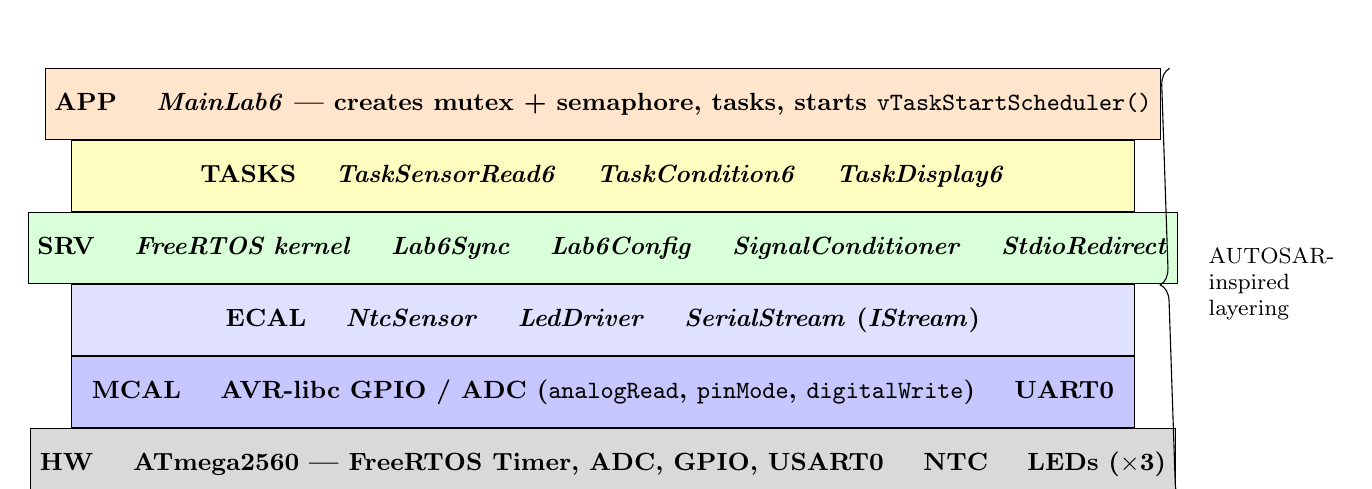
\begin{tikzpicture}[node distance=0pt]

  \def\LW{13.5cm}

  \node[layer, minimum width=\LW, fill=orange!20] (app)
    {\textbf{APP} \quad \textit{MainLab6} --- creates mutex + semaphore, tasks, starts \texttt{vTaskStartScheduler()}};

  \node[layer, minimum width=\LW, fill=yellow!25, below=of app] (tasks)
    {\textbf{TASKS} \quad \textit{TaskSensorRead6} \quad \textit{TaskCondition6} \quad \textit{TaskDisplay6}};

  \node[layer, minimum width=\LW, fill=green!15, below=of tasks] (srv)
    {\textbf{SRV} \quad \textit{FreeRTOS kernel} \quad \textit{Lab6Sync} \quad \textit{Lab6Config} \quad \textit{SignalConditioner} \quad \textit{StdioRedirect}};

  \node[layer, minimum width=\LW, fill=blue!12, below=of srv] (ecal)
    {\textbf{ECAL} \quad \textit{NtcSensor} \quad \textit{LedDriver} \quad \textit{SerialStream} (\textit{IStream})};

  \node[layer, minimum width=\LW, fill=blue!22, below=of ecal] (mcal)
    {\textbf{MCAL} \quad AVR-libc GPIO / ADC (\texttt{analogRead}, \texttt{pinMode}, \texttt{digitalWrite}) \quad UART0};

  \node[layer, minimum width=\LW, fill=gray!30, below=of mcal] (hw)
    {\textbf{HW} \quad ATmega2560 --- FreeRTOS Timer, ADC, GPIO, USART0 \quad NTC \quad LEDs ($\times$3)};

  \draw[decorate, decoration={brace, amplitude=6pt, mirror}]
    ([xshift=3pt]app.north east) -- ([xshift=3pt]hw.south east)
    node[midway, right=8pt, font=\footnotesize, align=left]
    {AUTOSAR-\\inspired\\layering};

\end{tikzpicture}
\caption{Layered Software Architecture}
\label{fig:layers}
\end{figure}

\begin{itemize}
  \item \textbf{APP}: \texttt{MainLab6} initialises hardware, creates \texttt{xLab6Mutex} and \texttt{xLab6NewSample}, creates three FreeRTOS tasks with differentiated priorities (sensor=3, conditioner=2, display=1), and starts the scheduler. \texttt{LoopLab6()} is empty --- never reached.
  \item \textbf{TASKS}: Three FreeRTOS task functions. The sensor reader is periodic (50\,ms) and signals the conditioner via a binary semaphore. The conditioner is event-driven, blocking until a new sample arrives. The display task is periodic (500\,ms).
  \item \textbf{SRV}: The FreeRTOS kernel provides scheduling, mutexes, semaphores, and \texttt{vTaskDelayUntil}. \texttt{Lab6Sync} declares the shared volatile data and synchronisation handles. \texttt{Lab6Config} holds all named constants. \texttt{SignalConditioner} provides the three conditioning algorithms. \texttt{StdioRedirect} connects \texttt{printf} to \texttt{SerialStream}.
  \item \textbf{ECAL}: \texttt{NtcSensor} wraps \texttt{analogRead()} and the Steinhart--Hart equation. \texttt{LedDriver} and \texttt{SerialStream} are reused from previous labs.
  \item \textbf{MCAL}: Arduino framework register-level abstractions, including ADC access.
  \item \textbf{HW}: Physical devices. Three LEDs provide visual status; the yellow LED blinks to indicate conditioning activity.
\end{itemize}

\subsection{Software Module Design}

% ── Mermaid source (render externally and save as images/lab6_modules.png) ──
% ```mermaid
% classDiagram
%     class IStream {
%         <<interface>>
%         +write(char c)*
%         +read() char*
%         +available() bool*
%     }
%     class SerialStream {
%         +begin(unsigned long baud)
%         +write(char c)
%         +read() char
%         +available() bool
%     }
%     class NtcSensor {
%         +InitializeNtcSensor(uint8_t pin)
%         +ReadNtcRaw(uint8_t pin) uint16_t
%         +NtcAdcToTempC(uint16_t adc) float
%         +NtcAdcToTempC10(uint16_t adc) int16_t
%     }
%     class LedDriver {
%         +InitializeLed(int pin)
%         +SetLedState(int pin, bool on)
%     }
%     class SignalConditioner {
%         +ApplySaturation(uint16_t val, min, max) uint16_t
%         +ApplyMedianFilter(uint16_t* buf, size) uint16_t
%         +ApplyWeightedAverage(uint16_t* buf, weights, size) uint16_t
%     }
%     class Lab6Config {
%         +NtcAnalogPin6 : A0
%         +GreenLedPin6 : 12
%         +RedLedPin6 : 11
%         +YellowLedPin6 : 10
%         +SaturationMin : 150
%         +SaturationMax : 900
%         +MedianWindowSize : 5
%         +WeightedAvgSize : 4
%         +WeightedAvgWeights : [50,25,15,10]
%         +AlertThresholdC : 30.0
%     }
%     class Lab6Sync {
%         +Lab6RawAdc : volatile uint16_t
%         +Lab6Saturated : volatile uint16_t
%         +Lab6MedianFiltered : volatile uint16_t
%         +Lab6WeightedAvg : volatile uint16_t
%         +Lab6TempC10 : volatile int16_t
%         +Lab6AlertActive : volatile bool
%         +xLab6Mutex : SemaphoreHandle_t
%         +xLab6NewSample : SemaphoreHandle_t
%     }
%     class TaskSensorRead6 {
%         +TaskSensorRead6Func(void*)
%     }
%     class TaskCondition6 {
%         -medianBuffer[5] : uint16_t
%         -avgBuffer[4] : uint16_t
%         +TaskCondition6Func(void*)
%     }
%     class TaskDisplay6 {
%         +TaskDisplay6Func(void*)
%     }
%     SerialStream ..|> IStream
%     TaskSensorRead6 --> NtcSensor : ReadNtcRaw
%     TaskSensorRead6 --> Lab6Sync : writes RawAdc, gives semaphore
%     TaskCondition6 --> Lab6Sync : takes semaphore, reads/writes data
%     TaskCondition6 --> SignalConditioner : pipeline stages
%     TaskCondition6 --> NtcSensor : NtcAdcToTempC10
%     TaskCondition6 --> LedDriver : SetLedState
%     TaskDisplay6 --> Lab6Sync : reads all shared data
% ```

\begin{figure}[H]
\centering
\includegraphics[width=0.85\textwidth]{images/lab6_modules.png}
\caption{Software Module Diagram}
\label{fig:modules}
\end{figure}

\subsection{FreeRTOS Task Synchronisation Diagram}

% ── Mermaid source (render externally and save as images/lab6_sequence.png) ──
% ```mermaid
% sequenceDiagram
%     participant T1 as Task1: SensorRead<br/>(50ms, prio 3)
%     participant SEM as xLab6NewSample<br/>(binary)
%     participant MTX as xLab6Mutex
%     participant SD as Shared Data<br/>(Lab6Sync)
%     participant T2 as Task2: Conditioner<br/>(event-driven, prio 2)
%     participant SC as SignalConditioner
%     participant LED as LEDs<br/>(G/R/Y)
%     participant T3 as Task3: Display<br/>(500ms, prio 1)
%
%     Note over T1: 50ms tick
%     T1->>T1: ReadNtcRaw(A0)
%     T1->>MTX: xSemaphoreTake()
%     T1->>SD: Lab6RawAdc = raw
%     T1->>MTX: xSemaphoreGive()
%     T1->>SEM: xSemaphoreGive()
%     SEM-->>T2: unblocks
%
%     T2->>MTX: xSemaphoreTake()
%     T2->>SD: read Lab6RawAdc
%     T2->>MTX: xSemaphoreGive()
%     T2->>SC: ApplySaturation(raw, 150, 900)
%     T2->>SC: ApplyMedianFilter(buffer, 5)
%     T2->>SC: ApplyWeightedAverage(buffer, weights, 4)
%     T2->>T2: NtcAdcToTempC10(weightedAvg)
%     T2->>LED: SetLedState(green/red/yellow)
%     T2->>MTX: xSemaphoreTake()
%     T2->>SD: write Saturated, Median, WAvg, TempC10, Alert
%     T2->>MTX: xSemaphoreGive()
%
%     Note over T3: 500ms tick
%     T3->>MTX: xSemaphoreTake()
%     T3->>SD: snapshot all fields
%     T3->>MTX: xSemaphoreGive()
%     T3->>T3: printf_P() status line
% ```

\begin{figure}[H]
\centering
\includegraphics[width=0.85\textwidth]{images/lab6_sequence.png}
\caption{FreeRTOS Task Synchronisation Sequence}
\label{fig:sequence}
\end{figure}

The synchronisation architecture:
\begin{itemize}
  \item \textbf{xLab6NewSample} (binary semaphore): Task~1 gives after storing a new raw ADC value; Task~2 blocks on take with \texttt{portMAX\_DELAY} --- zero CPU while waiting. This ensures the conditioning pipeline runs exactly once per new sample.
  \item \textbf{xLab6Mutex}: Protects all six shared volatile variables. Each task acquires the mutex only for the minimum duration needed to read or write shared data.
  \item \textbf{Priority assignment}: Task~1 (sensor read, prio~3) ensures timely ADC acquisition. Task~2 (conditioner, prio~2) runs immediately after being signalled. Task~3 (display, prio~1) yields to both processing tasks.
\end{itemize}

\subsection{Signal Conditioning Pipeline --- Block Diagram}

\begin{figure}[H]
\centering
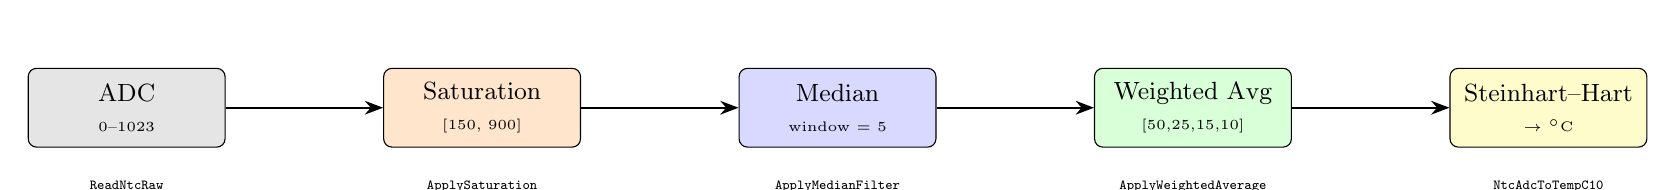
\begin{tikzpicture}[
  block/.style={rectangle, draw, rounded corners=3pt, minimum width=2.5cm, minimum height=1.0cm, align=center, font=\small},
  arr/.style={-Stealth, thick},
  node distance=2.0cm
]
  \node[block, fill=gray!20] (adc) {ADC\\{\tiny 0--1023}};
  \node[block, fill=orange!20, right=of adc] (sat) {Saturation\\{\tiny [150, 900]}};
  \node[block, fill=blue!15, right=of sat] (med) {Median\\{\tiny window = 5}};
  \node[block, fill=green!15, right=of med] (wavg) {Weighted Avg\\{\tiny [50,25,15,10]}};
  \node[block, fill=yellow!20, right=of wavg] (sh) {Steinhart--Hart\\{\tiny $\to$ $^{\circ}$C}};

  \draw[arr] (adc) -- (sat);
  \draw[arr] (sat) -- (med);
  \draw[arr] (med) -- (wavg);
  \draw[arr] (wavg) -- (sh);

  \node[below=0.3cm of adc, font=\tiny] {\texttt{ReadNtcRaw}};
  \node[below=0.3cm of sat, font=\tiny] {\texttt{ApplySaturation}};
  \node[below=0.3cm of med, font=\tiny] {\texttt{ApplyMedianFilter}};
  \node[below=0.3cm of wavg, font=\tiny] {\texttt{ApplyWeightedAverage}};
  \node[below=0.3cm of sh, font=\tiny] {\texttt{NtcAdcToTempC10}};

\end{tikzpicture}
\caption{Signal Conditioning Pipeline --- Block Diagram}
\label{fig:pipeline}
\end{figure}

Each stage operates on the output of the previous stage. All five stages execute within a single invocation of \texttt{TaskCondition6Func}, triggered by the binary semaphore from the sensor reader. The intermediate values (raw, saturated, median, weighted average, temperature) are stored in shared memory for the display task to report.

\subsection{Electronic Design}

\begin{figure}[H]
\centering
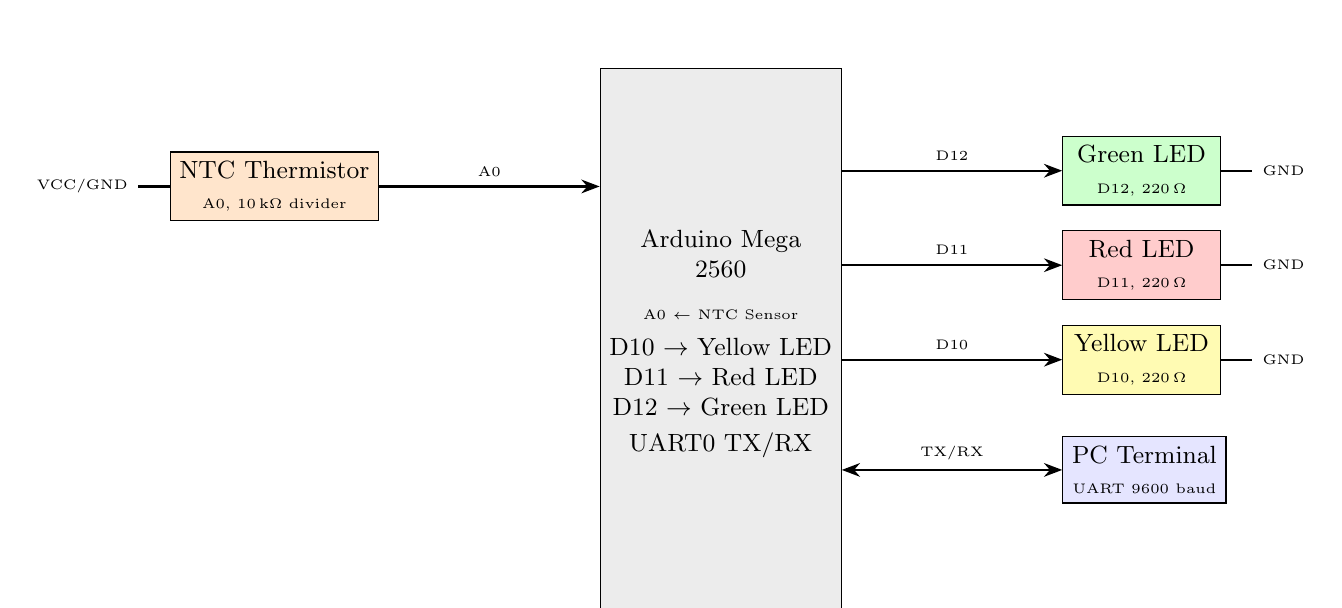
\begin{tikzpicture}[
  blk/.style={rectangle, draw, minimum height=1.4cm, align=center, font=\small},
  mcu/.style={blk, fill=gray!15, minimum width=3.0cm, minimum height=7.0cm},
  ledb/.style={blk, fill=green!20, minimum width=2.0cm, minimum height=0.75cm},
  ledr/.style={blk, fill=red!20,   minimum width=2.0cm, minimum height=0.75cm},
  ledy/.style={blk, fill=yellow!30, minimum width=2.0cm, minimum height=0.75cm},
  snsb/.style={blk, fill=orange!20, minimum width=2.0cm, minimum height=0.75cm},
  bus/.style={-Stealth, thick},
  lbl/.style={font=\tiny, midway},
]

  \node[mcu] (mcu) {Arduino Mega\\2560\\[4pt]
    \tiny A0 $\leftarrow$ NTC Sensor\\[2pt]
    D10 $\to$ Yellow LED\\D11 $\to$ Red LED\\D12 $\to$ Green LED\\[2pt]
    UART0 TX/RX};

  \node[snsb, left=2.8cm of mcu, yshift=2.0cm] (ntc)
    {NTC Thermistor\\{\tiny A0, 10\,k$\Omega$ divider}};

  \node[ledb, right=2.8cm of mcu, yshift=2.2cm] (gled)
    {Green LED\\{\tiny D12, 220\,$\Omega$}};

  \node[ledr, right=2.8cm of mcu, yshift=1.0cm] (rled)
    {Red LED\\{\tiny D11, 220\,$\Omega$}};

  \node[ledy, right=2.8cm of mcu, yshift=-0.2cm] (yled)
    {Yellow LED\\{\tiny D10, 220\,$\Omega$}};

  \node[blk, fill=blue!10, minimum width=2.0cm, minimum height=0.75cm, right=2.8cm of mcu, yshift=-1.6cm] (ser)
    {PC Terminal\\{\tiny UART 9600 baud}};

  \draw[bus] (ntc.east) -- node[lbl, above]{A0} (mcu.west |- ntc.east);

  \draw[bus] (mcu.east |- gled.west) -- node[lbl, above]{D12} (gled.west);
  \draw[bus] (mcu.east |- rled.west) -- node[lbl, above]{D11} (rled.west);
  \draw[bus] (mcu.east |- yled.west) -- node[lbl, above]{D10} (yled.west);
  \draw[bus, Stealth-Stealth] (mcu.east |- ser.west) --
    node[lbl, above]{TX/RX} (ser.west);

  \foreach \led in {gled, rled, yled}
    \draw[thick] (\led.east) -- ++(0.4,0) node[right, font=\tiny]{GND};

  \draw[thick] (ntc.west) -- ++(-0.4,0) node[left, font=\tiny]{VCC/GND};

\end{tikzpicture}
\caption{Electronic Design --- Pin Connection Diagram}
\label{fig:elec}
\end{figure}

\begin{itemize}
  \item \textbf{NTC Thermistor (A0)}: Connected in a voltage divider. VCC $\to$ $R_{fixed}$ (10\,k$\Omega$) $\to$ A0 $\to$ NTC $\to$ GND.
  \item \textbf{Green LED (D12)}: Normal state indicator. 220\,$\Omega$ series resistor. ON when conditioned temperature is below 30\,$^{\circ}$C.
  \item \textbf{Red LED (D11)}: Alert state indicator. Same resistor topology. ON when conditioned temperature exceeds 30\,$^{\circ}$C.
  \item \textbf{Yellow LED (D10)}: Conditioning activity indicator. Toggles on each conditioning cycle (every 50\,ms when samples arrive). 220\,$\Omega$ resistor.
  \item \textbf{UART0 (TX/RX)}: 9600\,baud serial connection for the 500\,ms status display.
\end{itemize}

% ─────────────────────────────────────────────────────────────────────────────
\section{Implementation}
% ─────────────────────────────────────────────────────────────────────────────

\subsection{Project Structure}

\begin{table}[H]
\centering
\begin{tabular}{@{}lp{8.2cm}@{}}
\toprule
\textbf{File} & \textbf{Purpose} \\
\midrule
\texttt{src/main.cpp}
  & Lab selector; dispatches \texttt{setup()}/\texttt{loop()} based on \texttt{ACTIVE\_LAB} \\
\texttt{src/labs/lab6/MainLab6.cpp}
  & Creates mutex + semaphore; creates three FreeRTOS tasks; calls \texttt{vTaskStartScheduler()} \\
\texttt{src/labs/lab6/TaskSensorRead6.cpp}
  & 50\,ms periodic ADC read; signals conditioner via semaphore \\
\texttt{src/labs/lab6/TaskCondition6.cpp}
  & Event-driven conditioning pipeline: sat $\to$ median $\to$ wavg $\to$ temp \\
\texttt{src/labs/lab6/TaskDisplay6.cpp}
  & 500\,ms periodic display of all pipeline values \\
\texttt{src/labs/lab6/SignalConditioner.cpp}
  & \texttt{ApplySaturation}, \texttt{ApplyMedianFilter}, \texttt{ApplyWeightedAverage} \\
\texttt{src/components/NtcSensor.cpp}
  & ADC read, Steinhart--Hart conversion \\
\texttt{src/components/LedDriver.cpp}
  & \texttt{InitializeLed} / \texttt{SetLedState} --- GPIO output \\
\texttt{src/components/SerialStream.cpp}
  & \texttt{IStream} implementation over \texttt{HardwareSerial} \\
\texttt{src/components/StdioRedirect.cpp}
  & \texttt{initStdio(IStream*)} via \texttt{fdev\_setup\_stream} \\
\texttt{include/labs/lab6/Lab6Config.h}
  & Named constants: pins, saturation limits, filter sizes, weights, timing \\
\texttt{include/labs/lab6/Lab6Sync.h}
  & Declares shared \texttt{volatile} data, mutex, and semaphore handles \\
\texttt{include/labs/lab6/SignalConditioner.h}
  & Conditioning function declarations \\
\texttt{include/drivers/NtcSensor.h}
  & NTC parameters ($R_0$, $T_0$, $B$, $R_{fixed}$); function declarations \\
\bottomrule
\end{tabular}
\caption{Project File Structure}
\label{tab:files}
\end{table}

\subsection{PlatformIO Environment Configuration}

The build is selected via the \texttt{[env:mega\_lab6]} environment in \texttt{platformio.ini}:

\begin{lstlisting}
[env:mega_lab6]
extends = env:mega
build_flags =
    -D USE_FREERTOS
    -D ACTIVE_LAB=6
\end{lstlisting}

This environment extends \texttt{env:mega}, inheriting the ATmega2560 board, Arduino framework, and \texttt{feilipu/FreeRTOS@\^{}10.5.1-1} dependency.

\subsection{Configuration Constants}

All configuration values are defined as named constants in \texttt{Lab6Config.h}:

\begin{lstlisting}[caption={Lab6Config.h --- configuration constants}]
const uint8_t NtcAnalogPin6  = A0;
const uint8_t GreenLedPin6   = 12;
const uint8_t RedLedPin6     = 11;
const uint8_t YellowLedPin6  = 10;

const uint16_t SaturationMin = 150;
const uint16_t SaturationMax = 900;

const uint8_t MedianWindowSize = 5;

const uint8_t  WeightedAvgSize = 4;
const uint16_t WeightedAvgWeights[WeightedAvgSize] =
    {50, 25, 15, 10};

const float AlertThresholdC = 30.0f;

const uint16_t SensorReadIntervalMs6  = 50;
const uint16_t ConditionIntervalMs6   = 50;
const uint16_t DisplayIntervalMs6     = 500;
\end{lstlisting}

\subsection{Shared Data and Synchronisation}

The shared state is declared in \texttt{Lab6Sync.h}:

\begin{lstlisting}[caption={Lab6Sync.h --- shared volatile data and sync handles}]
#pragma once
#ifdef USE_FREERTOS
#include <Arduino_FreeRTOS.h>
#include <semphr.h>

extern volatile uint16_t Lab6RawAdc;
extern volatile uint16_t Lab6Saturated;
extern volatile uint16_t Lab6MedianFiltered;
extern volatile uint16_t Lab6WeightedAvg;
extern volatile int16_t  Lab6TempC10;
extern volatile bool     Lab6AlertActive;

extern SemaphoreHandle_t xLab6Mutex;
extern SemaphoreHandle_t xLab6NewSample;
#endif
\end{lstlisting}

Six shared variables store the complete pipeline state, allowing the display task to report every intermediate value. The binary semaphore \texttt{xLab6NewSample} provides event-driven triggering of the conditioning task.

\subsection{Task Setup and Scheduler Launch}

\texttt{SetupLab6()} in \texttt{MainLab6.cpp} performs the following steps:
\begin{enumerate}
  \item Initialise serial at 9600\,baud and hook STDIO via \texttt{initStdio(\&SerialIo)}.
  \item Initialise the NTC sensor pin (A0) and three LEDs (D10, D11, D12).
  \item Set initial LED states: green ON, red OFF, yellow OFF.
  \item Create the mutex: \texttt{xLab6Mutex = xSemaphoreCreateMutex()}.
  \item Create the binary semaphore: \texttt{xLab6NewSample = xSemaphoreCreateBinary()}.
  \item Create three tasks with differentiated priorities: Sensor (128 words, prio~3), Conditioner (256 words, prio~2), Display (256 words, prio~1).
  \item Print a welcome message with pipeline configuration via \texttt{printf\_P}.
  \item Call \texttt{vTaskStartScheduler()} --- does not return.
\end{enumerate}

\begin{lstlisting}[caption={SetupLab6 --- task creation and scheduler launch}]
void SetupLab6() {
    SerialIo.begin(9600);
    initStdio(&SerialIo);

    InitializeNtcSensor(NtcAnalogPin6);
    InitializeLed(GreenLedPin6);
    InitializeLed(RedLedPin6);
    InitializeLed(YellowLedPin6);

    SetLedState(GreenLedPin6, true);
    SetLedState(RedLedPin6, false);
    SetLedState(YellowLedPin6, false);

    xLab6Mutex     = xSemaphoreCreateMutex();
    xLab6NewSample = xSemaphoreCreateBinary();

    xTaskCreate(TaskSensorRead6Func, "Sensor",
                128, nullptr, 3, nullptr);
    xTaskCreate(TaskCondition6Func,  "Condition",
                256, nullptr, 2, nullptr);
    xTaskCreate(TaskDisplay6Func,    "Display",
                256, nullptr, 1, nullptr);

    printf_P(PSTR("Lab 6: Analog Signal "
                  "Conditioning\n"));
    printf_P(PSTR("Sensor: NTC on A0\n"));
    printf_P(PSTR("Pipeline: Sat[%u-%u] -> "
        "Median[%u] -> WAvg[%u]\n"),
        SaturationMin, SaturationMax,
        MedianWindowSize, WeightedAvgSize);

    vTaskStartScheduler();
}
\end{lstlisting}

\subsection{Signal Conditioning Module}

The \texttt{SignalConditioner} module implements the three conditioning algorithms as stateless, reusable functions:

\begin{lstlisting}[caption={SignalConditioner --- saturation}]
uint16_t ApplySaturation(uint16_t value,
        uint16_t minVal, uint16_t maxVal) {
    if (value < minVal) return minVal;
    if (value > maxVal) return maxVal;
    return value;
}
\end{lstlisting}

\begin{lstlisting}[caption={SignalConditioner --- median filter (insertion sort)}]
uint16_t ApplyMedianFilter(uint16_t* buffer,
        uint8_t bufferSize) {
    uint16_t sorted[bufferSize];
    for (uint8_t i = 0; i < bufferSize; i++)
        sorted[i] = buffer[i];

    for (uint8_t i = 1; i < bufferSize; i++) {
        uint16_t key = sorted[i];
        int8_t j = i - 1;
        while (j >= 0 && sorted[j] > key) {
            sorted[j + 1] = sorted[j];
            j--;
        }
        sorted[j + 1] = key;
    }

    return sorted[bufferSize / 2];
}
\end{lstlisting}

\begin{lstlisting}[caption={SignalConditioner --- weighted moving average}]
uint16_t ApplyWeightedAverage(const uint16_t* buffer,
        const uint16_t* weights, uint8_t size) {
    uint32_t weightedSum = 0;
    uint32_t weightTotal = 0;

    for (uint8_t i = 0; i < size; i++) {
        weightedSum += (uint32_t)buffer[i]
                     * (uint32_t)weights[i];
        weightTotal += weights[i];
    }

    if (weightTotal == 0) return 0;
    return (uint16_t)(weightedSum / weightTotal);
}
\end{lstlisting}

The median filter copies the buffer to a local \texttt{sorted} array before sorting to preserve the circular buffer's insertion order. The weighted average uses 32-bit accumulation to avoid overflow when multiplying 16-bit values.

\subsection{TaskSensorRead6Func --- Sensor Acquisition}

The sensor task reads the ADC every 50\,ms, stores the raw value under mutex, and signals the conditioner:

\begin{lstlisting}[caption={TaskSensorRead6Func --- periodic sensor acquisition}]
void TaskSensorRead6Func(void* pvParameters) {
    const TickType_t Interval =
        pdMS_TO_TICKS(SensorReadIntervalMs6);
    TickType_t xLastWakeTime = xTaskGetTickCount();

    for (;;) {
        uint16_t raw = ReadNtcRaw(NtcAnalogPin6);

        xSemaphoreTake(xLab6Mutex, portMAX_DELAY);
        Lab6RawAdc = raw;
        xSemaphoreGive(xLab6Mutex);

        xSemaphoreGive(xLab6NewSample);

        vTaskDelayUntil(&xLastWakeTime, Interval);
    }
}
\end{lstlisting}

The raw ADC value is written to shared memory under mutex \emph{before} the semaphore is given, ensuring the conditioner always sees a valid sample when it wakes.

\subsection{TaskCondition6Func --- Conditioning Pipeline}

The conditioning task is event-driven: it blocks on the binary semaphore until a new sample arrives, then runs the full pipeline:

\begin{lstlisting}[caption={TaskCondition6Func --- event-driven conditioning pipeline}]
void TaskCondition6Func(void* pvParameters) {
    uint16_t medianBuffer[MedianWindowSize];
    uint16_t avgBuffer[WeightedAvgSize];
    uint8_t medianIdx = 0, avgIdx = 0;
    uint8_t medianFill = 0, avgFill = 0;

    for (uint8_t i = 0; i < MedianWindowSize; i++)
        medianBuffer[i] = 0;
    for (uint8_t i = 0; i < WeightedAvgSize; i++)
        avgBuffer[i] = 0;

    for (;;) {
        xSemaphoreTake(xLab6NewSample, portMAX_DELAY);

        xSemaphoreTake(xLab6Mutex, portMAX_DELAY);
        uint16_t raw = Lab6RawAdc;
        xSemaphoreGive(xLab6Mutex);

        // Stage 1: Saturation
        uint16_t saturated =
            ApplySaturation(raw,
                SaturationMin, SaturationMax);

        // Stage 2: Median filter
        medianBuffer[medianIdx] = saturated;
        medianIdx = (medianIdx + 1) % MedianWindowSize;
        if (medianFill < MedianWindowSize) medianFill++;

        uint16_t medianWork[MedianWindowSize];
        for (uint8_t i = 0; i < MedianWindowSize; i++)
            medianWork[i] = medianBuffer[i];
        uint16_t median =
            ApplyMedianFilter(medianWork, medianFill);

        // Stage 3: Weighted moving average
        avgBuffer[avgIdx] = median;
        avgIdx = (avgIdx + 1) % WeightedAvgSize;
        if (avgFill < WeightedAvgSize) avgFill++;

        uint16_t orderedBuf[WeightedAvgSize];
        for (uint8_t i = 0; i < avgFill; i++) {
            uint8_t idx = (avgIdx + WeightedAvgSize
                          - 1 - i) % WeightedAvgSize;
            orderedBuf[i] = avgBuffer[idx];
        }
        uint16_t weightedAvg =
            ApplyWeightedAverage(orderedBuf,
                WeightedAvgWeights, avgFill);

        // Stage 4: Temperature conversion
        int16_t tempC10 = NtcAdcToTempC10(weightedAvg);

        // Stage 5: Alert determination
        bool alert = (tempC10 >=
            (int16_t)(AlertThresholdC * 10.0f));

        SetLedState(GreenLedPin6, !alert);
        SetLedState(RedLedPin6,    alert);

        // Yellow LED toggles each cycle
        static bool yellowToggle = false;
        yellowToggle = !yellowToggle;
        SetLedState(YellowLedPin6, yellowToggle);

        xSemaphoreTake(xLab6Mutex, portMAX_DELAY);
        Lab6Saturated      = saturated;
        Lab6MedianFiltered = median;
        Lab6WeightedAvg    = weightedAvg;
        Lab6TempC10        = tempC10;
        Lab6AlertActive    = alert;
        xSemaphoreGive(xLab6Mutex);
    }
}
\end{lstlisting}

Key implementation details:
\begin{itemize}
  \item \textbf{Circular buffers}: Both the median and weighted average stages use circular buffers with separate index and fill counters. During the initial fill-up phase (\texttt{fill < size}), only the available samples are processed.
  \item \textbf{Ordered extraction}: The weighted average requires samples ordered from newest to oldest. The \texttt{orderedBuf} array is filled by walking backwards from the most recent insertion point.
  \item \textbf{Working copy}: The median filter operates on a copy (\texttt{medianWork}) of the circular buffer to avoid corrupting the insertion order during sorting.
  \item \textbf{Yellow LED}: Toggles on every conditioning cycle as a visual heartbeat, confirming the pipeline is active.
  \item \textbf{Simple threshold}: Unlike Lab~1.5, the alert uses a simple threshold (30\,$^{\circ}$C) without hysteresis or debounce, since the conditioning pipeline itself provides noise rejection.
\end{itemize}

\subsection{TaskDisplay6Func --- Pipeline Status Display}

The display task snapshots all pipeline intermediate values and emits a formatted status line every 500\,ms:

\begin{lstlisting}[caption={TaskDisplay6Func --- periodic pipeline status display}]
void TaskDisplay6Func(void* pvParameters) {
    const TickType_t Interval =
        pdMS_TO_TICKS(DisplayIntervalMs6);
    TickType_t xLastWakeTime = xTaskGetTickCount();

    for (;;) {
        vTaskDelayUntil(&xLastWakeTime, Interval);

        xSemaphoreTake(xLab6Mutex, portMAX_DELAY);
        uint16_t raw     = Lab6RawAdc;
        uint16_t sat     = Lab6Saturated;
        uint16_t med     = Lab6MedianFiltered;
        uint16_t wavg    = Lab6WeightedAvg;
        int16_t  tempC10 = Lab6TempC10;
        bool     alert   = Lab6AlertActive;
        xSemaphoreGive(xLab6Mutex);

        int16_t whole = tempC10 / 10;
        uint16_t frac = (uint16_t)(tempC10 < 0
            ? -(tempC10 % 10) : (tempC10 % 10));

        printf_P(PSTR("RAW:%u SAT:%u MED:%u "
            "AVG:%u T:%d.%uC %s\n"),
            raw, sat, med, wavg,
            whole, frac,
            alert ? "ALERT" : "OK");
    }
}
\end{lstlisting}

The output includes all pipeline intermediate values: raw ADC, saturated value, median-filtered value, weighted average, final temperature, and alert status. This allows observing the effect of each conditioning stage.

\subsection{STDIO Usage}

\begin{table}[H]
\centering
\begin{tabular}{@{}lp{4cm}p{5.5cm}@{}}
\toprule
\textbf{Function} & \textbf{Call site} & \textbf{Output} \\
\midrule
\texttt{printf\_P}
  & \texttt{SetupLab6} (3$\times$)
  & Welcome message, sensor info, pipeline configuration \\
\texttt{printf\_P}
  & \texttt{TaskDisplay6Func}
  & 500\,ms status: RAW, SAT, MED, AVG, temperature, alert \\
\bottomrule
\end{tabular}
\caption{STDIO Usage}
\label{tab:stdio}
\end{table}

\subsection{Code}

The full source code is available at the GitHub repository listed as the first entry in the bibliography \cite{code}.

% ─────────────────────────────────────────────────────────────────────────────
\section{Results}
% ─────────────────────────────────────────────────────────────────────────────

The application was verified in simulation and on hardware. The following scenarios were tested:

\begin{enumerate}
  \item \textbf{Welcome message}: On power-up, three lines are printed: ``Lab 6: Analog Signal Conditioning'', sensor type, and the pipeline configuration with saturation limits, median window, and weighted average size.

  \item \textbf{Normal operation}: With the sensor at room temperature, all pipeline stages produce consistent values. The green LED is ON, the display shows ``OK'', and the yellow LED blinks steadily.

  \item \textbf{Saturation clamping}: When the ADC value drops below 150 (simulating a sensor fault), the saturated value clamps to 150. Values above 900 clamp to 900.

  \item \textbf{Impulse noise rejection}: Injecting a brief spike in the ADC reading (e.g., one sample at 1023 among normal readings) is rejected by the median filter --- the output remains stable.

  \item \textbf{Smooth tracking}: Gradual temperature changes produce a smoothly varying weighted average, with the most recent sample contributing 50\% and older samples contributing progressively less.

  \item \textbf{Alert activation}: When the conditioned temperature exceeds 30\,$^{\circ}$C, the red LED activates and the display shows ``ALERT''. Since the pipeline filters noise, false alerts are eliminated.

  \item \textbf{Yellow LED heartbeat}: The yellow LED toggles on every conditioning cycle (every 50\,ms), confirming the pipeline is active.
\end{enumerate}

A sample serial monitor output:

\begin{lstlisting}
Lab 6: Analog Signal Conditioning
Sensor: NTC on A0
Pipeline: Sat[150-900] -> Median[5] -> WAvg[4]
RAW:512 SAT:512 MED:512 AVG:512 T:25.3C OK
RAW:510 SAT:510 MED:511 AVG:511 T:25.4C OK
RAW:1023 SAT:900 MED:512 AVG:511 T:25.4C OK
RAW:508 SAT:508 MED:510 AVG:510 T:25.5C OK
RAW:450 SAT:450 MED:508 AVG:494 T:27.2C OK
RAW:420 SAT:420 MED:450 AVG:462 T:29.5C OK
RAW:400 SAT:400 MED:420 AVG:425 T:31.8C ALERT
\end{lstlisting}

Note line~3: a spike to 1023 is clamped to 900 by saturation, and the median filter (512) rejects it entirely. The weighted average (511) barely changes, demonstrating effective noise rejection.

\subsection{Test Validation}

\begin{table}[H]
\centering
\begin{tabular}{@{}llp{7.5cm}@{}}
\toprule
\textbf{Test ID} & \textbf{Result} & \textbf{Observations} \\
\midrule
RF01\_T01  & Pass & ADC reads NTC value correctly every 50\,ms. \\
RF02\_T01  & Pass & Saturation clamps out-of-range values to [150, 900]. \\
RF03\_T01  & Pass & Median filter rejects impulse noise spikes. \\
RF04\_T01  & Pass & Weighted average smooths signal with correct weight distribution. \\
RF05\_T01  & Pass & Steinhart--Hart conversion produces accurate temperature. \\
RF06\_T01  & Pass & Display shows all pipeline intermediate values every 500\,ms. \\
RF07\_T01  & Pass & Green/Red LEDs correctly reflect alert status. \\
RF08\_T01  & Pass & Yellow LED toggles on each conditioning cycle. \\
RNF01\_T01 & Pass & Tasks run concurrently; no shared data corruption observed. \\
RNF02\_T01 & Pass & Code is modular with separate files per component. \\
RNF03\_T01 & Pass & Mutex protects all shared volatile variables. \\
RNF04\_T01 & Pass & Binary semaphore synchronises sensor-to-conditioner handoff. \\
RNF05\_T01 & Pass & All configuration values are named constants. \\
RNF06\_T01 & Pass & SignalConditioner functions are stateless and reusable. \\
RNF07\_T01 & Pass & PROGMEM strings conserve SRAM on ATmega2560. \\
\bottomrule
\end{tabular}
\caption{Test Results for the Signal Conditioning Application}
\label{tab:tests}
\end{table}

% ─────────────────────────────────────────────────────────────────────────────
\section{Note on AI}
% ─────────────────────────────────────────────────────────────────────────────

\hspace{0.8cm}
For this laboratory work, AI assistants such as Claude~4.6~Sonnet were used for explaining code sections, underlying technologies (median filtering, weighted moving averages, signal conditioning theory), and for assisting with debugging. They were also used for paraphrasing and structuring ideas in this report. All AI-generated content was reviewed and verified against the actual implementation.

% ─────────────────────────────────────────────────────────────────────────────
\section{Conclusion}
% ─────────────────────────────────────────────────────────────────────────────

\hspace{0.8cm}
This laboratory work demonstrated analog signal conditioning using a multi-stage pipeline on an ATmega2560 with FreeRTOS. The raw NTC thermistor reading passes through saturation (clamping to [150, 900]), median filtering (window of 5 samples), and weighted moving averaging (weights 50/25/15/10) before Steinhart--Hart temperature conversion. Each stage addresses a specific noise or fault condition: saturation rejects sensor faults, the median filter eliminates impulse noise, and the weighted average smooths the signal.

\hspace{0.8cm}
The producer-consumer architecture --- where the sensor reader signals the conditioner via a binary semaphore --- ensures that the pipeline processes exactly one sample per acquisition cycle with zero CPU waste while waiting. Unlike Lab~1.5, which used hysteresis and debouncing for noise-resistant threshold alerting, Lab~1.6 relies on the conditioning pipeline itself to produce a clean signal, allowing a simple threshold comparison for alert determination.

\hspace{0.8cm}
The \texttt{SignalConditioner} module encapsulates the three conditioning algorithms as stateless, reusable functions, separate from the FreeRTOS task logic. This separation enables independent testing and reuse in other contexts. The display task reports all intermediate pipeline values, providing full observability of the conditioning process. This architecture demonstrates the complete signal acquisition and conditioning chain from raw ADC reading to calibrated temperature output.

% ─────────────────────────────────────────────────────────────────────────────
\section{Bibliography}
% ─────────────────────────────────────────────────────────────────────────────

\begingroup
\makeatletter
\renewcommand{\section}[2]{}
\makeatother

\begin{thebibliography}{}

  \bibitem{code}
  \url{https://github.com/NeValetik/si-labs}

  \bibitem{ntc_steinhart}
  Ametherm. \textit{NTC Thermistors --- Steinhart and Hart Equation}.
  \url{https://www.ametherm.com/thermistor/ntc-thermistor-steinhart-hart-equation}

  \bibitem{median_filter}
  Smith, S.\,W. \textit{The Scientist and Engineer's Guide to Digital Signal Processing}, Chapter~15: Moving Average Filters.
  \url{http://www.dspguide.com/ch15.htm}

  \bibitem{freertos_sem}
  FreeRTOS. \textit{Binary Semaphores}.
  \url{https://www.freertos.org/Documentation/02-Kernel/02-Kernel-features/02-Queues-mutexes-and-semaphores/02-Binary-semaphores}

  \bibitem{freertos_mutex}
  FreeRTOS. \textit{Mutexes}.
  \url{https://www.freertos.org/Documentation/02-Kernel/02-Kernel-features/02-Queues-mutexes-and-semaphores/04-Mutexes}

  \bibitem{pio}
  PlatformIO. \textit{PlatformIO Documentation --- atmelavr Platform}.
  \url{https://docs.platformio.org/en/latest/platforms/atmelavr.html}

  \bibitem{avr}
  Microchip Technology. \textit{ATmega2560 Datasheet}, DS40002211A, 2020.
  \url{https://ww1.microchip.com/downloads/en/devicedoc/atmel-2549-8-bit-avr-microcontroller-atmega640-1280-1281-2560-2561_datasheet.pdf}

\end{thebibliography}
\endgroup

\pagebreak
\end{document}
